\documentclass[11pt]{article}
\textheight 22cm \textwidth 16.5cm \oddsidemargin 0cm \topmargin -.5cm
\usepackage[utf8x]{inputenc}
\usepackage{pricing_notes}

\date{Lecture 4 (5 Feb. 2013)}

\begin{document}

{\small \maketitle}

\section{Recapitulation}
We discussed the price of a (European call) option as a function 
$$C(t, S(t); r, \sigma; K, T)$$
where $t$ (date) and $S(t)$ (underlying price) are state variables, $r$ (short-term interest rate) and $\sigma$ (volatility) are model parameters, and $K$ (strike price) and $T$ (maturity) characterise the option. We defined the at-the-money (ATM) strike as $K_{ATM} = S(t)$\\

\begin{remark}
Consider holding a European call option maturing at $T > t$ (i.e. without possibility of exercise), and the price of that option at $t$ compared with the theoretical return $\left(S(t) -K\right)^+$ on exercise at that time. We call this value  the {\em intrinsic value} of the option, and can decompose the proce $C(t)$ into the instrinsic value plu some {\em time value} dependent on the time to expiry and the volatility of the underlying price.
\end{remark}

\section{History of Volatility Models}

As of 1973, market practitioners started the practice of taking market prices for given options and solving for $\sigma$ to get the {\em implied volatility}. Given liquidity consideations, the market practise was to use out-of-the-money (OTM) options to calculate volatility: i.e., using the call option price when $K > S(t)$ and using the put option price when $K < S(t)$. \\

Between 1975 and 1979, market practitioners observed a flat volatility structure, with identical implied volatilities across all strikes. \\

Between 1981 and 1987, the volatility structure was observed to curve upwards symmetrically around the ATM point. The proposed explanation was that sellers of OTM options demanded reward for holding a perceived higher risk. This perceived risk was in contradiction to the pure Black-Scholes model, and theoreticians began to enhance the model. \\

In 1986, Wiggins introduced stochastic volatility, turning the constant $\sigma$ into a stochastic process $\sigma(t)$. The volatility was now a state variable of the option price:
$$C(t, S(t), \sigma(t); r; K, T)$$

\begin{remark}
When introducing stochastic volatility into the model, if there are no (sufficiently liquid) primitive securities that can be used to hedge $\sigma(t)$, then the market will not be complete, unlike the world of stochastic interest rates, where there are many instruments with which to hedge $r(t)$.
\end{remark}

In 1987 Hull and White introduced the following correlated volatility model:
\begin{align*}
\frac{\dif S(t)}{S(t)} &= \mu \dif t + \sigma(t) \dif W_1(t) \\
\frac{\dif \sigma(t)}{\sigma(t)} &= \eta \dif t + \xi \dif W_2(t) \\
\dif W_1(t) \dif W_2(t) &= \rho \dif t
\end{align*}
where the expected correlation of $\dif W_1$ and $\dif W_2$ was negative. Two options for the drift term for $\sigma$ could be ruled out immediately: the case of positive drift (in which case volatility could increase without bound) or the case of negative drift (in which case volatility could decrease below zero). In other words, $\eta$ muse be equal to zero. \\

After the market crash in 1987, in was widely understood that the market behaved differently during negative movement than during positive movement. Sellers of puts demanded a higher return for their risk, and academics noticed that the volatility smile was no longer symmetric: \\

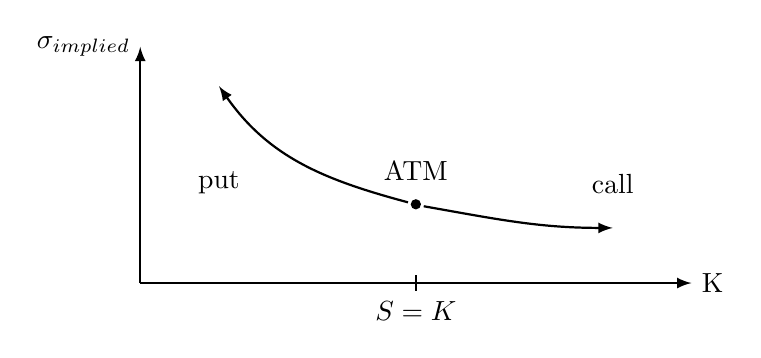
\begin{tikzpicture}[thick]
    \draw [-latex] (0,0) to (7,0) node [right] {K};
    \draw [-latex] (0,0) to (0,3) node [left] {$\sigma_\text{implied}$};
    \draw [-latex] (3.6,0.975) to [out=-10,in=180] (6,0.7);
    \node [above] at (6,1) {call};
    \draw [-latex] (3.4,1.025) to [out=165,in=-55] (1,2.5);
    \node [above] at (1,1) {put};
    \draw [fill] (3.5,1) circle [radius=0.05] node [above=5] {ATM};
    \draw (3.5,0.1) to (3.5,-0.1) node [below] {$S=K$};
\end{tikzpicture} \\

The difference between the put and call volatilities of similar deltas was called the skew. In equities the most common shape was reverse skew (put options displayed higher implied volatilities than call options). The opposite (forward skew) is more common incommodities. \\

Another empirical observation regarding volatility is that it tends to be mean reverting. To accomodate this, in 1991, Stein and Stein (a father and son team) proposed a different form of stochastic volatility following a mean-reverting Ornstein-Uhlenbeck process:
$$ \dif \sigma(t) = a\left(b-\sigma(t)\right) + c \dif W^2_t \quad \text{where} \quad a,b,c > 0$$
This allows for mean-reverting volatility, but still suffered from the flaw that it could produce a negative volatility. \\

In 1993, Heston proposed the "Heston model," which is still popular today:
\begin{align*}
\frac{\dif S(t)}{S(t)} &= \mu \dif t + \sigma(t) \dif W_1(t) \\
\frac{\dif \sigma(t)}{\sigma(t)} &= u (v - \Sigma)\dif t + x \sqrt{\Sigma}\dif W_2(t) \\
\dif W_1(t) \dif W_2(t) &= \rho \dif t
\end{align*}
where $\rho < 0$. This sort of process was first introduces by Cox, Ingersoll, and Ross in 1985 to model the short-term interest rate, and is mean-reverting without the possibility of negative outcomes (for certain values of $u$, $v$, and $x$). However, the model was much more mathematically involved. \\

In 1993, Geman and Yor produced a paper on Bessel processes, Asian options, and perpetuities in which they showed that that the Cox-Ingersoll-Ross square-root processes are related to Bessel processes, and gave a more rigorous foundation to Heston's results. \\

In 1994, Dupire and (separately) Derman and Kani introduced the local volatilty model, to avoid the incompleteness created by $\sigma(t)$ being a process of its own. Suppose $S$ is a non-dividend-paying stock with the following price process under $\Qmeas$:
$$\dif S(t) = r S(t) \dif t + \sigma \left( S(t) \right) \dif \widehat{W}_t$$
In this model, $\sigma(t)$ is a deterministic function of $S$. The calibration of the model boils down to finding and parametrising that function using the market prices of vanilla options.

\begin{remark}
This model is not used to make money trading vanilla options. However, once the model is calibrated, it can be used to trade more complicated options usch as barrier, Asian, and other exotic products.
\end{remark}

By 1998, market practitioners had begun incorporating maturities beyond 6 months into their models. They had also begun to use the $\Qmeas_T$ measure and to use the maturity forward price for the underlying of the option, i.e. for an option $C^T$ expiring at $T$, to use the $T$-forward price of $S$, $f^T_S(t)$.

\begin{remark}
A brief reminder of notation. The forward price $f^T_S(t)$ is defined as 
$$ f^T_S(t) = \frac{S(t)}{B^T(t)}$$
To represent Brownian motion under different measures, we use the following notation:
\begin{align*}
\text{under} \Pmeas: \qquad \dif W_t \\
\text{under} \Qmeas: \qquad \dif \widehat{W}_t \\
\text{under} \Qmeas_T: \qquad \dif \widehat{\widehat{W}}_t \\
\end{align*}
\end{remark}

In 2002, Hagan {\em et al.} proposed the "stochastic alpha, beta, rho" (SABR) model that fully included the $\Qmeas_T$ measure and the notion of forward price martingales:
\begin{align*}
\dif f^T_S(t) &= 0 \dif t + \sigma(t)\left[ f_S^T(t) \right]^\alpha \dif \widehat{\widehat{W}}_1(t) \\
\dif \sigma(t) &= 0 \dif t + \beta \sigma(t) \widehat{\widehat{W}}_2(t) \\
\dif \widehat{\widehat{W}}_1(t) \dif \widehat{\widehat{W}}_2(t) &= \rho \dif t \\
\end{align*}
The authors proposed a numerical method to extract the parameters ($\alpha$, $\beta$, and $\rho$) from observed option prices.

\section{Discontinuous Prices}

Back in 1976, Merton had already observed that continuity of price trajectories was too strong an assumption: share prices did not, in practice, follow geometric Brownian motion. He proposed (under $\Pmeas$):
$$ \frac{\dif S(t)}{S(t)} = \mu \dif t + \sigma \dif W_t + U \dif N(t)$$
where $N(T) \sim \operatorname{Poisson}(\lambda)$, where $\lambda > 0$ and $U$ is the multiplier of $S(t)$ when the jump occurs. Merton knew of no hedging instrument for the jump risk, and assumed that the market price of jump risk was zero. This model is not used because, at the very least, the market does in fact positively price the risk of down jumps. \\

So far, to explain the skew, we have navigated between stochastic volatility, local volatility, and jumps. We observed that in all cases, models were applied under $\Pmeas$, $\Qmeas$, or $\Qmeas_T$. \\

In 1999-2001, Geman, Madan, and Yor proposed pure-jump processes to model $S$ under $\Pmeas$ and $\Qmeas$. The motivation for this was that the observed market price of  stocks was discontinuous, and pure jump models were in good agreement with observed characteristics of the price process. \\

Lévy had already studied certain pure jump processes that made computation feasible, and these formed the basis for the new price process. In 2002 Carr, Geman, Madan, Yor proposed a pure jump Lévy process known as CGMY (or {\em tempered stable}). One of the attractions of this type of pocess was that it made it possible to reproduce price trajectories with four parametrisable moments (mean, variance, skew, kurtosis) rather than only the first two (as in the normal distribution). \\

CGMY was good for modelling skew, but did not replicate the observed term structure of volatility. In 2003, the CGMY process was extended with stochastic volatility as a solution to this problem, and in 2004, Hagan proposed CGMY as an alternative to SABR. \\

\begin{remark}
In stock markets, high volumes and down moves are associated with higher volatility. In commodities, the reverse is true: higher prices and lower volumes are associated with higher volatility.
\end{remark}

\section{Asian Options}
In 1989, with European and American options already well established, a new form of option payoff was proposed: the Asian option. As date $t$, consider an option $C^{As}$ with the payoff
\begin{align*}
C^{\text{As}}(T) &\equiv \max \left( 0, \operatorname{Avg}(T) - K\right) \\
\text{where} \quad \operatorname{Avg}(T) &\equiv \frac{S(t_1) + S(t_2) + \cdots + S(t_n)}{n}
\end{align*}
with $t_n = T$. In practice, this option was very popular in new and less developed markets, where $S(T)$ was subject to manipulation at or around the expiry $T$. The average price over a number of periods was harder to manipulate. Also, in the FX markets, it may be necessary to hedge an average exchange rate across a series of cash flows of similar size; an Asian option would not be a perfect hedge, but may be cheaper than hedging each flow individually. \\

To price Asian options, we begin with the same process:
\begin{align*}
\text{under} \Qmeas: \qquad \frac{\dif S(t)}{S(t)} &= (r - g) \dif t + \sigma \dif \widehat{W}_t \\
S(t_j) &= S_0 \exp \left\{ (r-g)(t_j-0) - \frac{\sigma^2}{2}t_j + \sigma \widehat{W}_{t_j}\right\} \\
A(T) &= \frac{1}{n} \sum{S(t_j)} \\ 
C^{\text{As}}(0) &= e^{-rt} \Exp_{\Qmeas} \left[ \left( A(T)-K \right)^+ \middle/ \Filtr_t \right]\\
\end{align*}
Since $A(T)$ is the sum of log-normally distributed processes, it is not itself log-normally distributed, so calculating the expectation is not as simple as in the previous cases. \\

In 1990, Kemna and Vorst proposed an approximation: to replace the arithmetic average $A(T)$ with the geometric average $A^{\text{Geom}}(T) = \sqrt[n]{\prod{S(t_j)}}$. This substitution has a closed form solution, but is only an approximation. Because 
$$\sqrt[n]{\prod x_i} \leqslant \frac{1}{n}\sum x_i$$
we know that $C^{\text{As}}(0) > C^{\text{Geom}}(0)$, which gives us a lower bound on the Asian option price, but we have no upper bound. \\

Practitioners then began pricing Asian options with Monte Carlo methods. Since the value of an Asian option is path-dependent, they needed to build price trajectories across all the observation points. Starting from $S(0)$, we can construct each successive $S(t)$ by 
$$S(t_i) = S(t_{i-1}) \exp \left\{ \left( (r-g) - \frac{\sigma}{2} \right)(t_i - t_{i-1}) + \sigma \widehat{W}(t_i - t_{i-1}) \right\}$$ \\

We denote this sequence $\Filtr_1 = \left\{ S(t) \right\}_{t=0,\dots,T}$ and calculate the average, which we denote $A_1(T)$, and calculate the payoff $a_i = \left( A(t) - K\right)^+$ . We can then construct $n$ such sequences (and their payoffs), and estimate the $C^{\text{As}}$ by
$$C^{\text{As}} \approx e^{-rt} \frac{\sum_{i=1}^n a_i}{n}$$
This gives us the Monte Carlo price of an Asian option.\\

If we want to hedge such an option, we will also need to calculate the delta of the option, $\pd{C^{\text{As}}}{S}$. Since we do not have a closed-form solution for the delta, we can use the finite difference method. Consider the value $C^{\text{As}}$ of the option as a function of $S$. At time $t$ and for a given $S(t)$ we can calculate the price at two nearby points $S(t) \pm \epsilon$, and draw the secant line between the two points:\\

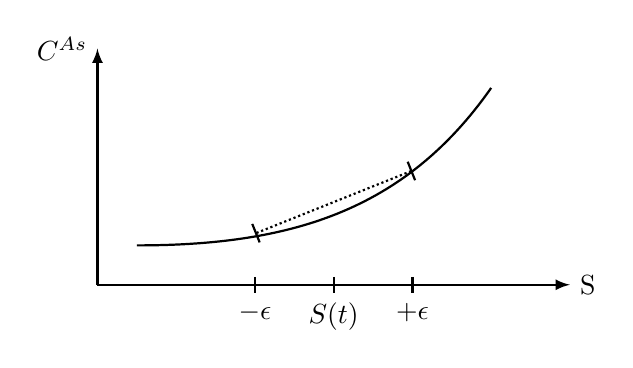
\begin{tikzpicture}[thick]
    \usetikzlibrary[arrows]
    \draw [-latex] (0,0) to (6,0) node [right] {S};
    \draw [-latex] (0,0) to (0,3) node [left] {$C^{\text{As}}$};
    \draw (0.5,0.5) to [out=0,in=-125] (5,2.5);
    \draw [densely dotted,arrows=|-|] (2, 0.65) to (4,1.45);
    \draw (2,0.1) to (2,-0.1) node [below] {$- \epsilon$};
    \draw (3,0.1) to (3,-0.1) node [below] {$S(t)$};
    \draw (4,0.1) to (4,-0.1) node [below] {$+ \epsilon$};
\end{tikzpicture} \\

By the mean value theorem, there exists a point on the curve between $S(t) + \epsilon$ and $S(t) - \epsilon$ where the tangent line is parallel to the secant line, i.e., that the delta of the option is equal to the slope of the line. By narrowing the distance between the two points, we can approximate the delta as closely as we choose (within numerical limits).









\end{document}
